% =============================================================================
% Supporting Information for
% "Universal power law decay of sequential influence in human language generation"
% Elan Barenholtz
% =============================================================================
% This is the SI Appendix stub. PNAS publishes SI as a separate PDF.
% Use the PNAS SI template (\templatetype{pnassupportinginfo}). Fill in the
% expanded methods and the SI tables/figures referenced from the main text.
% =============================================================================

\documentclass[9pt,twoside,lineno]{pnas-new}

\templatetype{pnassupportinginfo}

\title{Universal power law decay of sequential influence in human language generation}
\author{Elan Barenholtz}
\correspondingauthor{Elan Barenholtz. E-mail: ebarenholtz@fau.edu}

\graphicspath{{Paper_Figures/}}

\begin{document}

\maketitle

% =============================================================================
% EXPANDED METHODS
% =============================================================================

\section*{Expanded Methods}

\subsection*{Corpora and preprocessing}
Wikipedia corpora were drawn from the most recent dumps available at the time of analysis. For each language, 60 articles were sampled at random subject to a minimum-length filter of 500 tokens after preprocessing. Articles were stripped of markup, references, and infobox content; only running prose was retained. Tokenization was performed by the probe model's native tokenizer for each analysis. The Buckeye Corpus comprises 26 speakers in spontaneous sociolinguistic interviews; only interviewee turns were retained, and 30-token target regions were sampled from continuous interviewee speech with at least 100 tokens of preceding context. The French Oral Narrative Corpus (Queen's University Belfast) comprises 87 stories from 17 storytellers; tokenization and target sampling followed the Buckeye procedure.

AI-generated corpora were produced with Claude Sonnet, prompted to write Wikipedia-style articles on topics drawn from the matched human Wikipedia corpora. Topic prompts and full generation parameters are provided in Section~\ref{sec:ai-prompts}.

\subsection*{Probe models and quantization}
Llama-3-8B-Instruct and Mistral-7B-v0.1 were loaded in 4-bit NF4 quantization via bitsandbytes on a single H100 GPU. Greedy decoding was not used; perplexity was computed analytically from the model's softmax over the target tokens. Neither model was fine-tuned for this study.

\subsection*{Influence measurement}
For each document, three target regions of 30 tokens were selected at the 25\%, 50\%, and 75\% positions in the document. For each target, context was revealed one token at a time from $c = 1$ to $c = 100$. At each $c$, target perplexity was computed under intact context (the actual preceding $c$ tokens, original order) and shuffled context (the same $c$ tokens in random order; per-document shuffles, fixed seed). The marginal at distance $d$ is $m_d = \text{perplexity}_{d-1} - \text{perplexity}_d$; the corrected marginal is $\Delta_d = m^{\text{intact}}_d - m^{\text{shuffled}}_d$.

Corrected marginals were aggregated across documents within each corpus and binned by distance. Power law ($\alpha \cdot d^{\beta}$), exponential ($\alpha \cdot e^{-\beta d}$), stretched exponential ($\alpha \cdot e^{-\beta d^{\gamma}}$), and logarithmic ($\alpha + \beta \log d$) functions were fit to the binned curve via nonlinear least squares on log-transformed data. Initialization, bin edges, and convergence diagnostics are detailed in Section~\ref{sec:fit-details}. Model comparison used AIC and BIC computed from log-likelihood under Gaussian residuals.

\subsection*{Sensitivity analyses}
Position invariance was verified by comparing exponents fit separately to the 25\%, 50\%, and 75\% target positions; no systematic position effect was observed (Section~\ref{sec:sensitivity}). Document-length invariance was verified by stratifying corpora into short, medium, and long subsamples and refitting; exponents agreed within $\pm 0.05$ across strata. Bin-choice sensitivity was verified by repeating fits with logarithmic bin spacing and with linear bin spacing; the qualitative model-comparison outcomes were preserved.

\subsection*{AI-generation prompts}
\label{sec:ai-prompts}
[Place full prompt text here.]

\subsection*{Fitting initialization and convergence}
\label{sec:fit-details}
[Place details here.]

\subsection*{Sensitivity analyses (full)}
\label{sec:sensitivity}
[Place full per-corpus sensitivity tables and panels here.]

% =============================================================================
% SI TABLES
% =============================================================================

\section*{SI Tables}

\begin{table*}[h]
\centering
\caption{Absolute coherence magnitude across distance bins (Llama-3-8B). Corrected marginal values at short (1--2 tokens), mid (10--15 tokens), and long (30--50 tokens) ranges. AI-generated text collapses to the floor at long range; human text retains substantial influence.}
\label{tab:absolute-magnitude}
\begin{tabular}{lrrrr}
\toprule
Dataset & Short (1--2) & Mid (10--15) & Long (30--50) & $\alpha$ \\
\midrule
Chinese Wiki     & 3.91 & 1.09 & 0.203 & $-0.77$ \\
Arabic Wiki      & 3.29 & 1.63 & 0.174 & $-0.79$ \\
Korean Wiki      & 1.61 & 0.99 & 0.128 & $-0.73$ \\
Japanese Wiki    & 3.06 & 0.91 & 0.106 & $-0.81$ \\
Turkish Wiki     & 1.96 & 0.85 & 0.068 & $-0.88$ \\
Finnish Wiki     & 1.26 & 0.43 & 0.047 & $-0.77$ \\
Buckeye spoken   & 3.47 & 1.73 & 0.237 & $-0.87$ \\
French spoken    & 2.36 & 1.24 & 0.156 & $-0.70$ \\
\midrule
Chinese AI       & 1.69 & 0.75 & 0.052 & $-0.93$ \\
English AI       & 2.27 & 0.93 & 0.030 & $-1.40$ \\
Turkish AI       & 1.65 & 0.72 & 0.029 & $-1.09$ \\
\bottomrule
\end{tabular}
\end{table*}

\begin{table*}[h]
\centering
\caption{Functional-form comparison by AIC. Column "Best fit" gives the functional form with the lowest AIC for each dataset--probe combination. $\Delta$AIC is best minus power law; negative values indicate the power law is preferred. Across 16 conditions, the power law is selected in 12 (75\%); the exponential form is never selected by Llama-3-8B.}
\label{tab:functional-form}
\begin{tabular}{llrrr}
\toprule
Dataset (Probe) & Best fit & $R^2$ (power) & $R^2$ (best) & $\Delta$AIC \\
\midrule
Chinese Wiki (Llama)    & Power law       & 0.92 & 0.83 & $-8.96$  \\
Japanese Wiki (Llama)   & Power law       & 0.84 & 0.65 & $-9.56$  \\
Korean Wiki (Llama)     & Stretched exp.  & 0.92 & 0.91 & $-1.85$  \\
Turkish Wiki (Llama)    & Power law       & 0.93 & 0.86 & $-7.88$  \\
Arabic Wiki (Llama)     & Power law       & 0.84 & 0.71 & $-7.40$  \\
Finnish Wiki (Llama)    & Power law       & 0.84 & 0.65 & $-9.59$  \\
Buckeye (Llama)         & Power law       & 0.94 & 0.84 & $-12.16$ \\
French spoken (Llama)   & Power law       & 0.77 & 0.69 & $-3.48$  \\
Chinese Wiki (Mistral)  & Exponential     & 0.78 & 0.84 & $+3.98$  \\
Japanese Wiki (Mistral) & Power law       & 0.86 & 0.78 & $-5.88$  \\
Korean Wiki (Mistral)   & Power law       & 0.86 & 0.82 & $-3.06$  \\
Turkish Wiki (Mistral)  & Power law       & 0.87 & 0.75 & $-8.07$  \\
Arabic Wiki (Mistral)   & Power law       & 0.85 & 0.82 & $-2.08$  \\
Finnish Wiki (Mistral)  & Exponential     & 0.85 & 0.86 & $+0.84$  \\
Buckeye (Mistral)       & Logarithmic     & 0.79 & 0.80 & $+0.88$  \\
French spoken (Mistral) & Power law       & 0.83 & 0.68 & $-7.48$  \\
\bottomrule
\end{tabular}
\end{table*}

% =============================================================================
% SI FIGURES
% =============================================================================

\section*{SI Figures}

\begin{figure}[h]
\centering
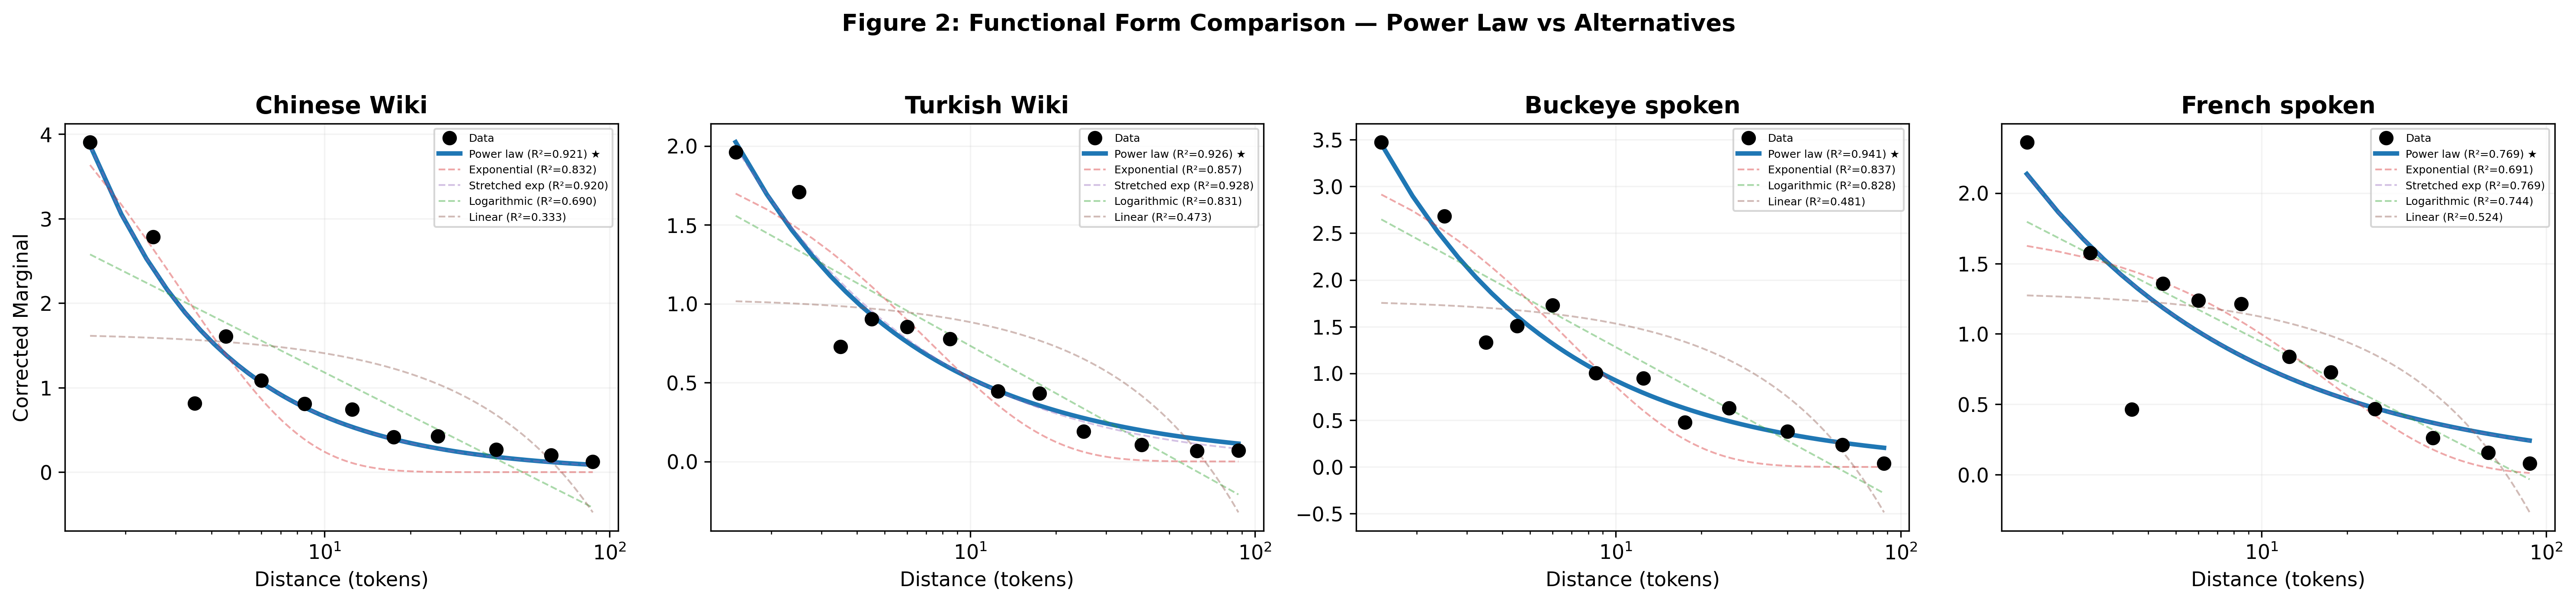
\includegraphics[width=\linewidth]{fig2_functional_form.png}
\caption{Functional-form comparison. Power law, exponential, stretched exponential, and logarithmic fits to the corrected-marginal curve for each dataset--probe combination, ranked by AIC. Power law is the overall winner in 12 of 16 cases; the exponential form is never selected by the better-calibrated probe (Llama-3-8B).}
\label{fig:functional-form}
\end{figure}

\begin{figure}[h]
\centering
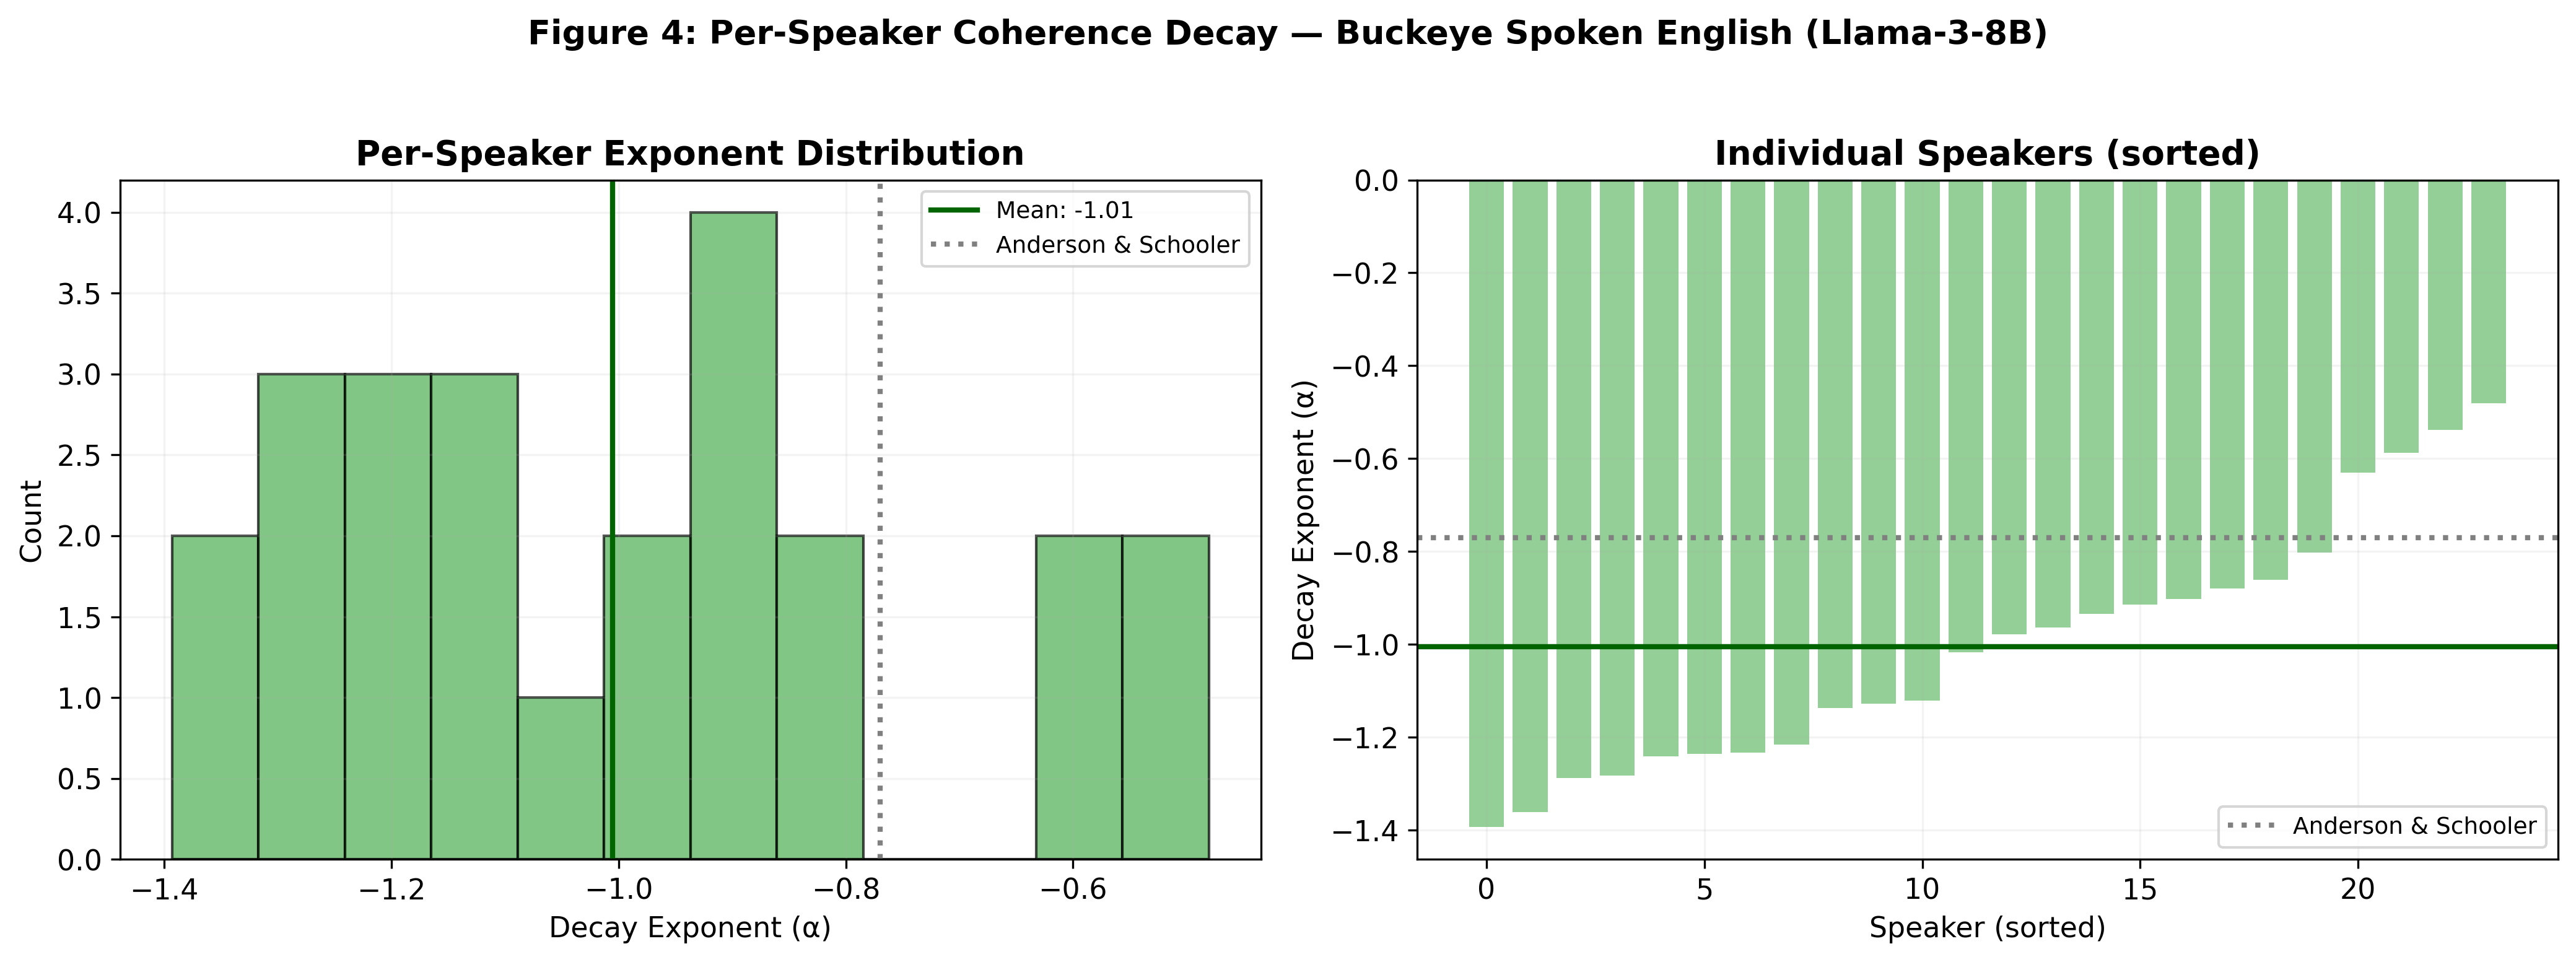
\includegraphics[width=\linewidth]{fig4_per_speaker.png}
\caption{Per-speaker influence-decay exponents in the Buckeye Corpus of Conversational Speech. Distribution of single-speaker exponents (Llama-3-8B) across 26 speakers, with matched AI value indicated. Zero overlap between human-speaker distribution and AI value.}
\label{fig:per-speaker}
\end{figure}

\begin{figure}[h]
\centering
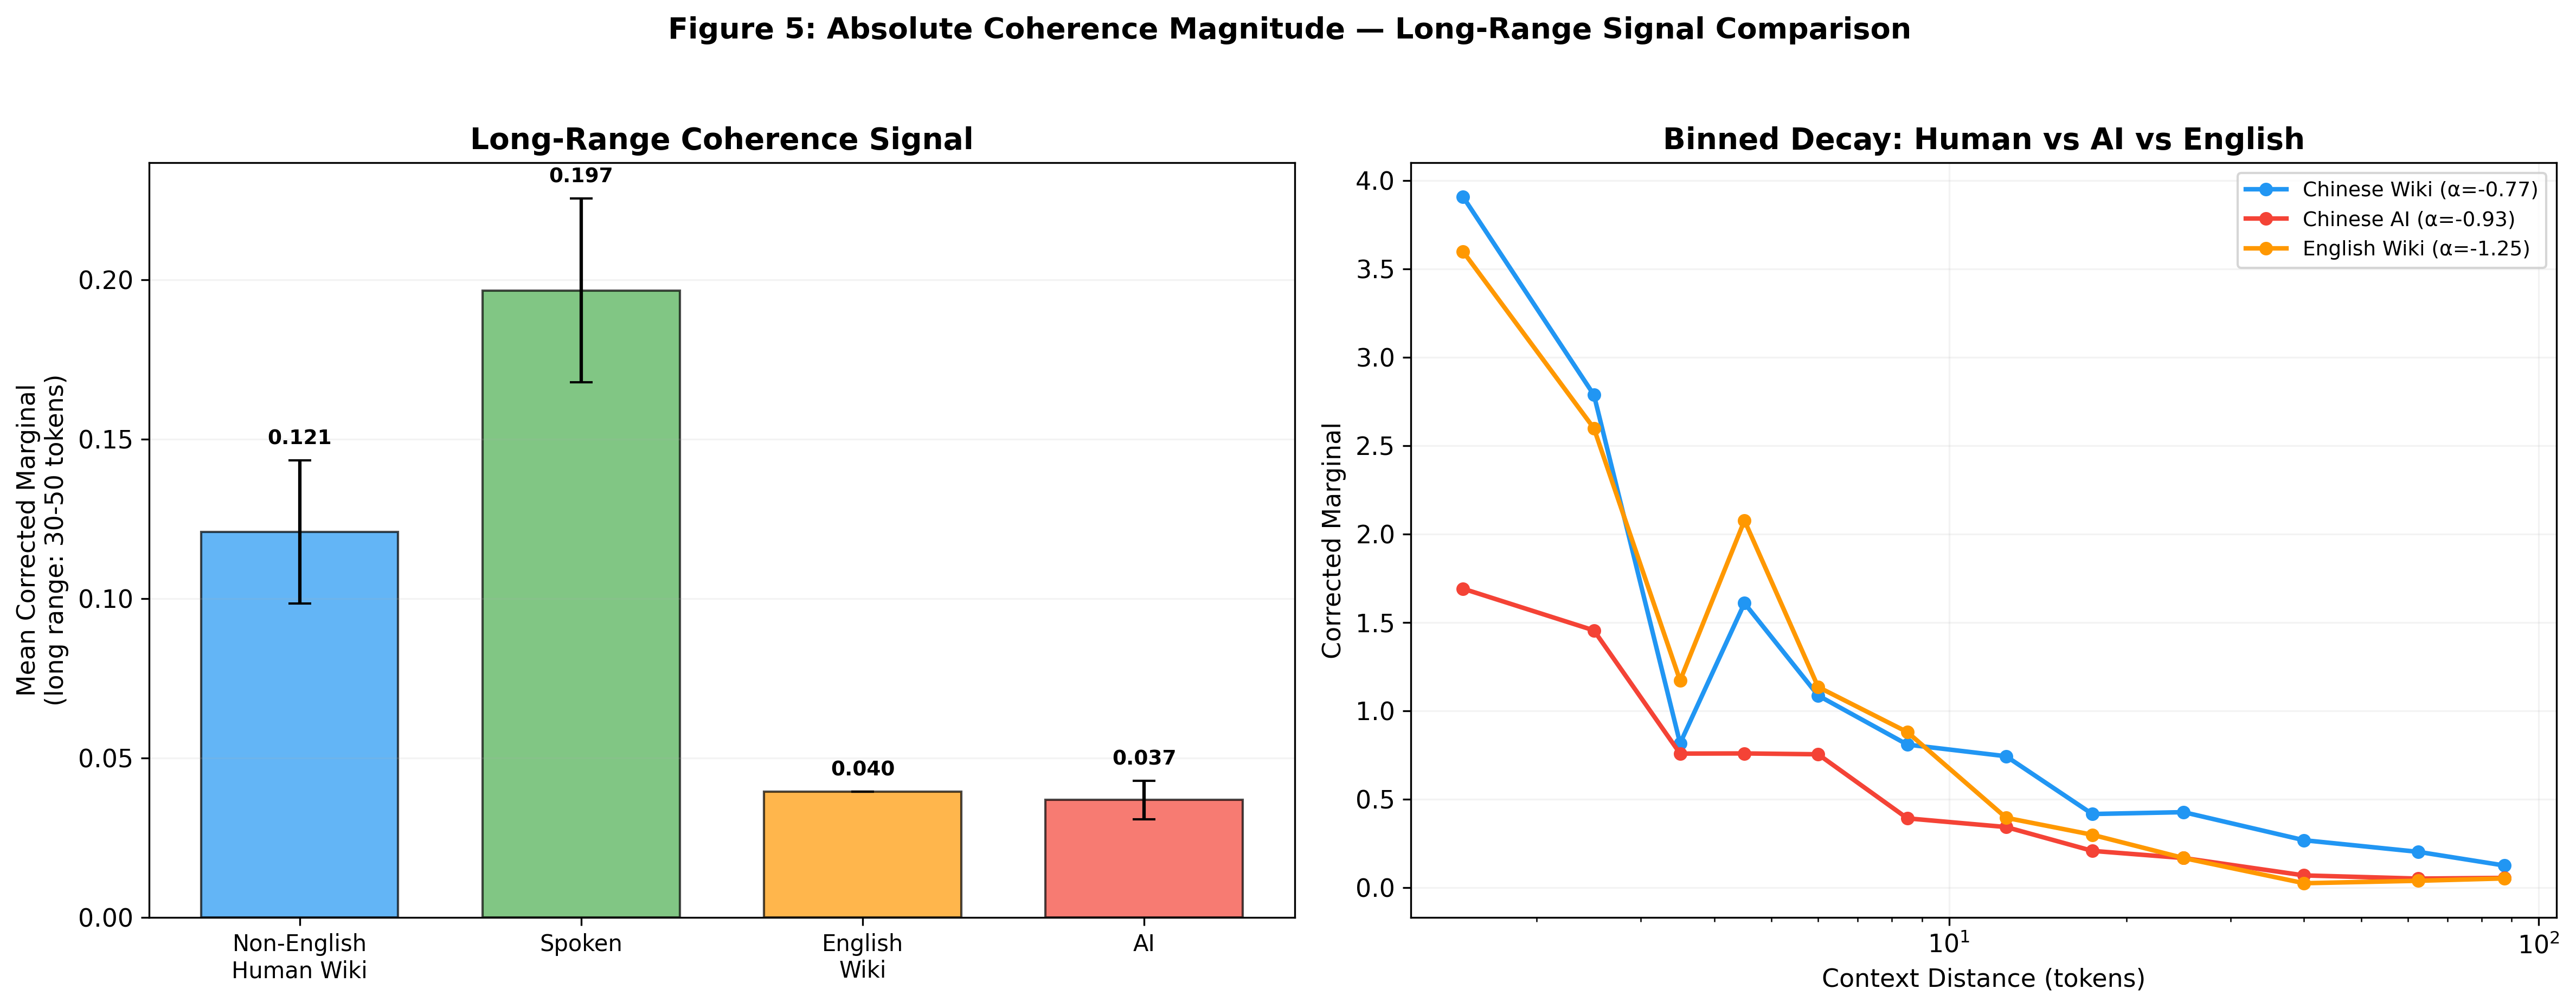
\includegraphics[width=\linewidth]{fig5_absolute_magnitude.png}
\caption{Absolute long-range coherence magnitude. Corrected marginal at the long-range bin (30--50 tokens) for human and matched AI corpora, showing the categorical separation between the two distributions.}
\label{fig:absolute-magnitude}
\end{figure}

\bibliography{references}

\end{document}
